\documentclass[10pt,aspectratio=169]{beamer}

\usetheme{Madrid}
\usepackage[T1]{fontenc}
\usepackage[utf8]{inputenc}
\usepackage{amsmath,amssymb}
\usepackage{booktabs}
\usepackage{graphicx}
\usepackage{xcolor}

\definecolor{accent}{HTML}{2563EB}
\definecolor{accent2}{HTML}{DC2626}
\definecolor{accent3}{HTML}{059669}
\definecolor{good}{HTML}{059669}
\definecolor{bad}{HTML}{DC2626}

\setbeamercolor{frametitle}{bg=accent,fg=white}
\setbeamertemplate{itemize item}{\textcolor{accent}{$\bullet$}}
\setbeamertemplate{navigation symbols}{}
\setbeamertemplate{footline}[frame number]

\title{Neural Survival Models: LongitudinalDeepHit}
\subtitle{Part E(iii) --- Transformer Encoder for Competing Risks}
\author{Yueqi Lin}
\institute{MTH 9877 --- Baruch College, Spring 2026}
\date{May 13, 2026}

% =========================================================================
\begin{document}

% ---- Title ---------------------------------------------------------------
\begin{frame}[plain]
    \titlepage
\end{frame}

% ---- 1. Motivation -------------------------------------------------------
\begin{frame}{Why go beyond Cox? Mortgage prepayment is path-dependent.}
    \begin{columns}[T,onlytextwidth]
        \column{0.48\textwidth}
        \begin{block}{Cox / Andersen-Gill limitations}
        \small
        \begin{itemize}\itemsep4pt
            \item Proportional hazards: covariate effect is \textbf{constant over time}
            \item Single scalar score — cannot model the \textbf{S-curve shape} of prepayment
            \item Competing risks require separate model fits; no shared representation
            \item Cannot exploit the \textbf{sequence structure} of monthly covariate history
        \end{itemize}
        \end{block}

        \column{0.48\textwidth}
        \begin{block}{What a sequence model can do}
        \small
        \begin{itemize}\itemsep4pt
            \item Read the full monthly path $[\mathbf{x}_1, \dots, \mathbf{x}_T]$ --- \textbf{burnout is encoded}
            \item Produce nonlinear, time-varying hazard rates $\lambda_k(t \mid \mathbf{x})$
            \item Model prepayment and default \textbf{jointly} via shared encoder
            \item Attention weights identify \textbf{which months} drive the prediction
        \end{itemize}
        \end{block}
    \end{columns}
\end{frame}

% ---- 2b. Architecture rationale ------------------------------------------
\begin{frame}{Why this architecture? Three design decisions.}
    \begin{columns}[T,onlytextwidth]
        \column{0.46\textwidth}
        \begin{alertblock}{Alternatives rejected}
        \small
        \begin{itemize}\itemsep4pt
            \item \textbf{LSTM} --- vanishing gradients at $T{=}120$; attends only to adjacent months; hard to interpret
            \item \textbf{Single-context head} --- no time index in head; near-constant hazard curve; gradient flows only through last hidden state
            \item \textbf{Two separate models} --- violates independent censoring (defaulted loans are riskiest borrowers, not random exits); loses shared macro signal
        \end{itemize}
        \end{alertblock}

        \column{0.50\textwidth}
        \begin{block}{Why this combination}
        \small
        \begin{itemize}\itemsep4pt
            \item \textbf{Causal Transformer} --- reaches any past month in one attention step; gradient flows through every position; weights are interpretable
            \item \textbf{Per-timestep head} --- $\lambda(t){=}\text{head}(h_t)$: hazard conditioned on full causal history $\mathbf{x}_1\!\dots\mathbf{x}_t$; every month trained independently
            \item \textbf{Joint encoder} --- shared representation captures that the same macro shock raises default and suppresses prepayment; chain product enforces $\text{CIF}_1{+}\text{CIF}_2{+}S{=}1$
        \end{itemize}
        \end{block}
    \end{columns}
\end{frame}

% ---- 3. Architecture -----------------------------------------------------
\begin{frame}{LongitudinalDeepHit: Transformer encoder with two CIF output heads.}
    \begin{columns}[T,onlytextwidth]
        \column{0.52\textwidth}
        \begin{block}{Architecture}
        \small
        \begin{tabular}{@{}ll@{}}
            \textbf{Input}  & $(B,\, T_{\max}{=}120,\, D{=}13)$ padded sequences \\
            \textbf{Proj.}  & Linear $D \to d_{\text{model}}{=}64$ \\
            \textbf{PE}     & Sinusoidal positional encoding on loan age \\
            \textbf{Enc.}   & $\times 2$ pre-norm layers, 4 heads, causal mask \\
            \textbf{Head 1} & FC $64\!\to\!64\!\to\!1$ per $h_t$, Sigmoid $\Rightarrow \lambda_1(t)$ \\
            \textbf{Head 2} & FC $64\!\to\!64\!\to\!1$ per $h_t$, Sigmoid $\Rightarrow \lambda_2(t)$ \\
            \textbf{CIFs}   & Competing-risk chain product \\
        \end{tabular}
        \end{block}

        \vspace{0.1em}
        \begin{block}{Competing-risk CIFs}
        \footnotesize
        \vspace{-0.9em}
        \begin{align*}
            \text{CIF}_k(t) &= \textstyle\sum_{s=1}^{t} \lambda_k(s)\cdot S(s-1) \\[-3pt]
            S(t) &= \textstyle\prod_{s=1}^{t}(1-\lambda_1(s))(1-\lambda_2(s))
        \end{align*}
        \vspace{-0.9em}
        Guarantees $\text{CIF}_1 + \text{CIF}_2 + S = 1$ at every $t$.
        \end{block}

        \column{0.44\textwidth}
        \begin{block}{Training objective}
        \small
        \vspace{-0.2em}
        \[
            \mathcal{L} = \mathcal{L}_{\text{NLL}} + \alpha\,\mathcal{L}_{\text{rank}},
            \quad \alpha=0.2
        \]
        \vspace{-0.2em}
        \textbf{NLL}: discrete-time cause-specific likelihood\\[2pt]
        \textbf{Ranking}: soft pairwise concordance (DeepHit-style)\\[4pt]
        \begin{tabular}{@{}ll@{}}
            Params & 76,290 \\[1pt]
            Data   & 101K loans, 4.5M rows \\[1pt]
            Epochs & 41 \;(best ep.\,29) \\[1pt]
            LR     & $3\!\times\!10^{-4}$, cosine \\[1pt]
            Loss   & $11.30 \to 11.28$ \\[1pt]
            Rank   & $1.97 \to 1.84$ \\
        \end{tabular}
        \end{block}
    \end{columns}
\end{frame}

% ---- 3. Training curves --------------------------------------------------
\begin{frame}{NLL collapses to $\lambda\!\approx\!0$; ranking loss drives AUC improvement.}
    \begin{center}
        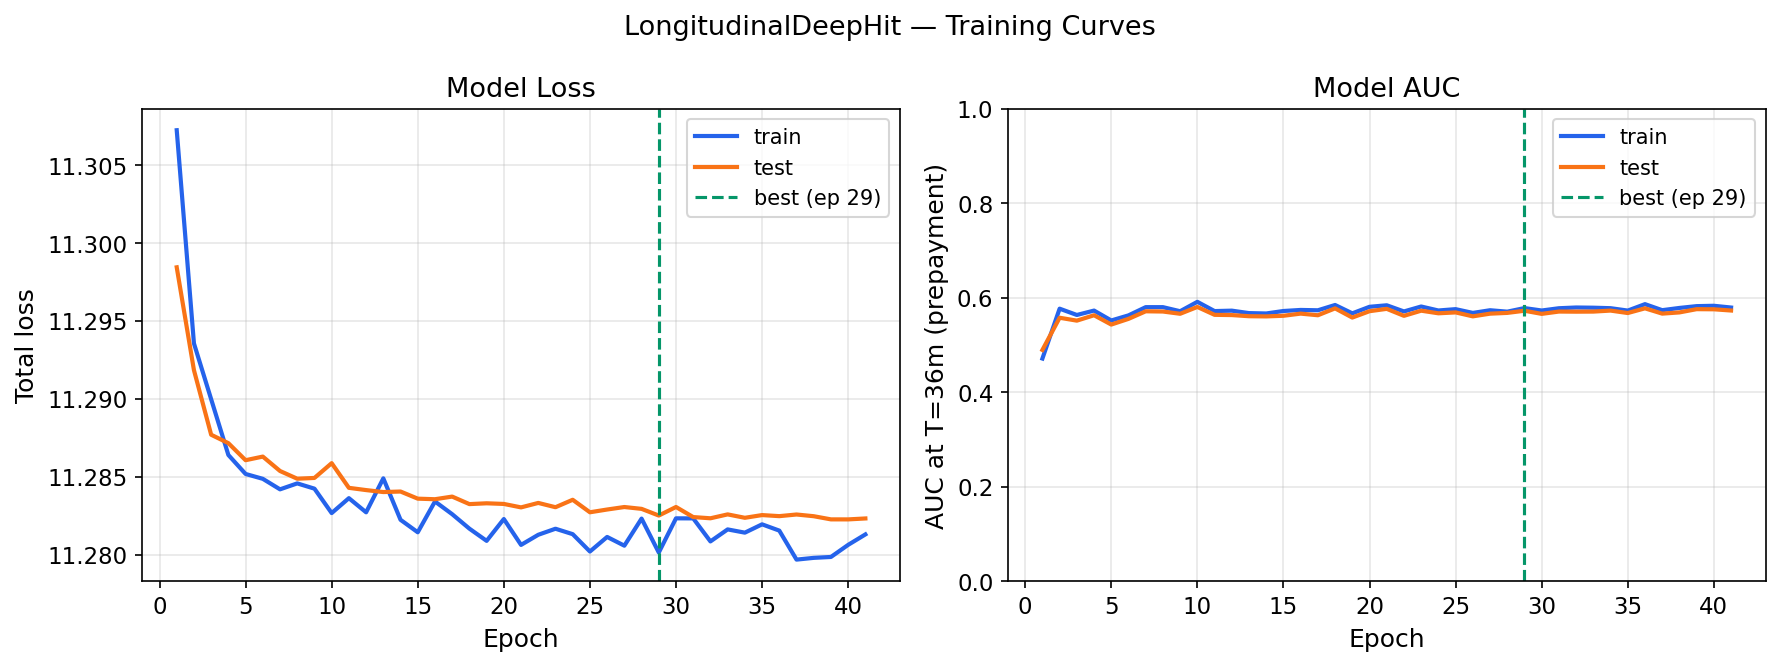
\includegraphics[width=0.92\linewidth]{processed/Eiii_training_curves}
    \end{center}
\end{frame}

% ---- 5. Gradient sensitivity ---------------------------------------------
\begin{frame}{Rate incentive and current LTV dominate prepayment; FICO dominates default.}
    \begin{center}
        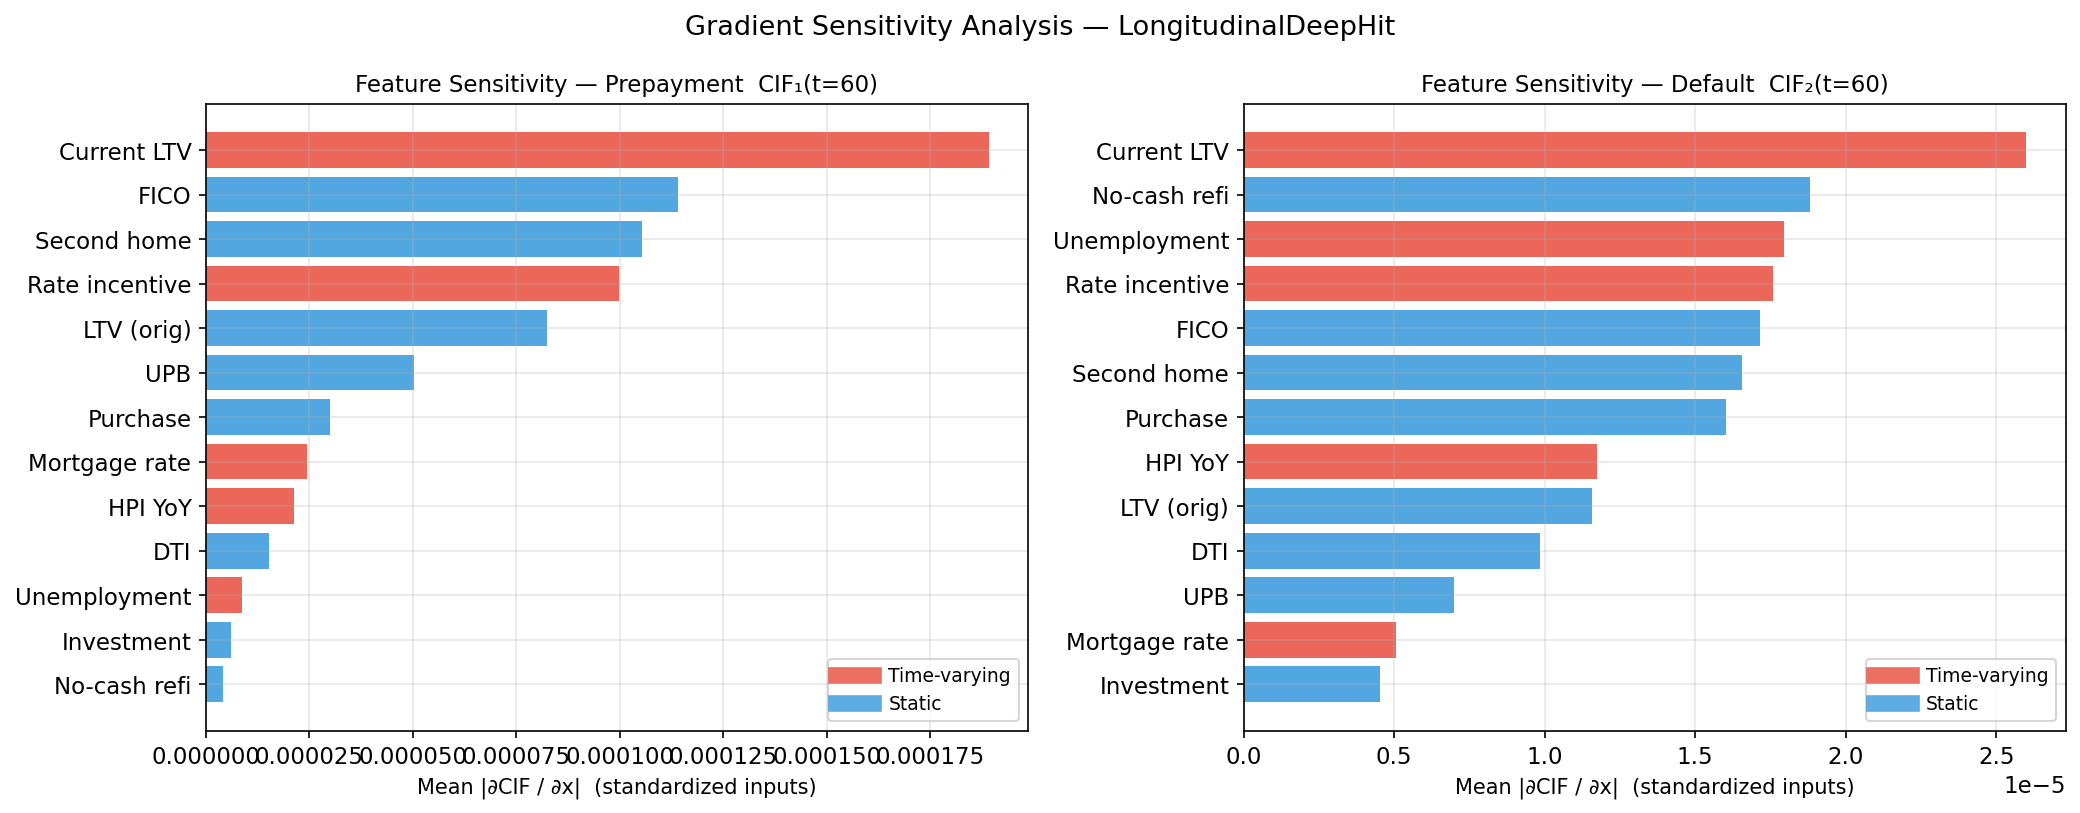
\includegraphics[width=0.84\linewidth]{processed/Eiii_gradient_sensitivity}
    \end{center}
    \vspace{-0.4em}
    \begin{center}
        \small
        \textcolor{bad}{Red} = time-varying features. \quad \textcolor{accent}{Blue} = static features.\\
        Dynamic features rank above static for prepayment; FICO and unemployment lead for default ---
        consistent with cause-specific Cox in E(i).
    \end{center}
\end{frame}

% ---- 6. Sensitivity over time --------------------------------------------
\begin{frame}{Feature importance shifts across the loan lifecycle --- unique to sequence models.}
    \begin{center}
        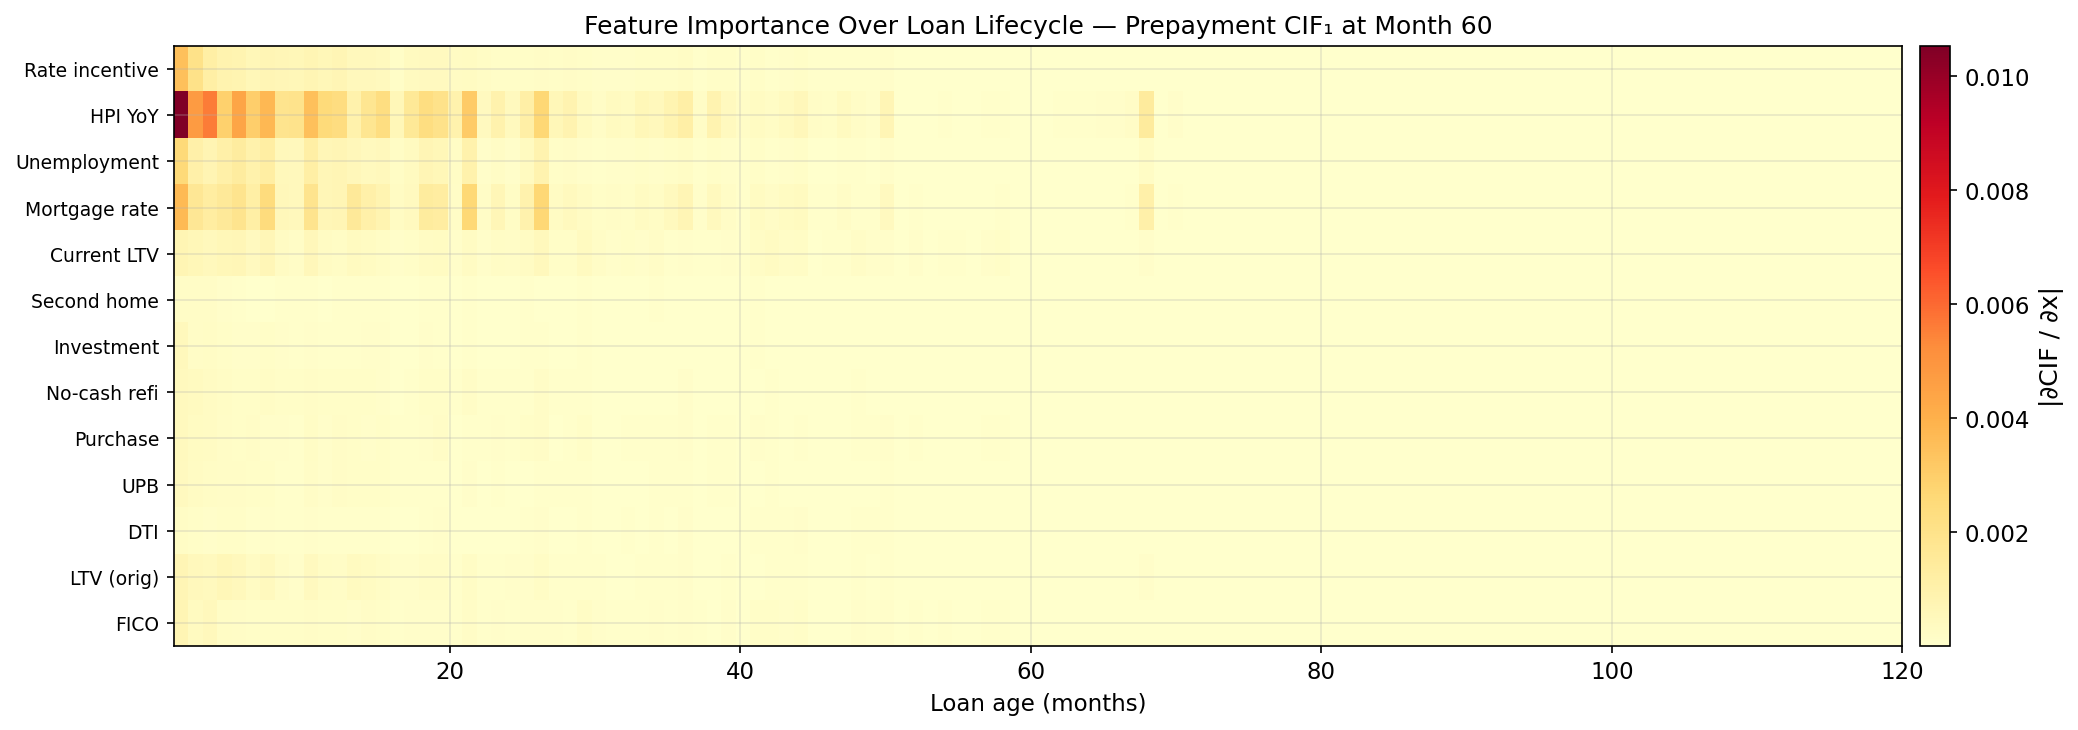
\includegraphics[width=0.92\linewidth]{processed/Eiii_sensitivity_over_time}
    \end{center}
    \vspace{-0.4em}
    \begin{center}
        \small
        \texttt{rate\_incentive} dominates early months; \texttt{Current LTV} rises as equity
        accumulates and gates the refi option. \texttt{Mortgage rate} is dark throughout ---
        the model learns the incentive \emph{spread} matters, not the rate level.
    \end{center}
\end{frame}

% ---- 7. Model performance ------------------------------------------------
\begin{frame}{Default AUC matches DeepCox; prepayment underperforms due to NLL collapse.}
    \begin{center}
        \small\textbf{Prepayment CIF$_1$ — AUC at fixed horizons}\\[4pt]
        \begin{tabular}{lcccc}
            \toprule
            \textbf{Model} & \textbf{T=12} & \textbf{T=24} & \textbf{T=36} & \textbf{T=60} \\
            \midrule
            Part D DeepCox$^\dagger$ & 0.684 & 0.701 & 0.721 & 0.729 \\
            DeepHit (20K)$^\ddagger$ & 0.641 & 0.622 & 0.572 & 0.515 \\
            DeepHit (344)$^\S$       & 0.677 & 0.647 & 0.565 & 0.334 \\
            \bottomrule
        \end{tabular}

        \vspace{8pt}
        \small\textbf{Default CIF$_2$ — AUC at fixed horizons}\\[4pt]
        \begin{tabular}{lcccc}
            \toprule
            \textbf{Model} & \textbf{T=12} & \textbf{T=24} & \textbf{T=36} & \textbf{T=60} \\
            \midrule
            Part D DeepCox$^\dagger$  & 0.684 & 0.701 & 0.721 & 0.729 \\
            DeepHit (20K)$^\ddagger$  & \textbf{0.687} & \textbf{0.708} & \textbf{0.707} & \textbf{0.726} \\
            \bottomrule
        \end{tabular}
        \vspace{3pt}\\
        \tiny $^\dagger$\,597K canonical\enspace
               $^\ddagger$\,20K hold-out\enspace
               $^\S$\,344 canonical loans
    \end{center}

    \vfill
    \begin{center}
        \small
        Default AUC \textbf{matches DeepCox} at every horizon with \textbf{6$\times$ fewer} training loans ---
        temporal covariate history compensates for data volume.
    \end{center}
\end{frame}

% ---- 8. Key Takeaways ----------------------------------------------------
\begin{frame}{Key Takeaways}
    \begin{enumerate}\itemsep10pt
        \item \textbf{Default AUC roughly matches DeepCox}\\
              Using 6$\times$ fewer training loans.
              Temporal covariate history compensates for data volume.

        \item \textbf{Gradient sensitivity independently replicates Cox findings}\\
              \texttt{rate\_incentive} + \texttt{Current LTV} drive prepayment;
              \texttt{FICO} + \texttt{unemployment} drive default --- recovered from data, not imposed.

        \item \textbf{Feature importance shifts across the loan lifecycle}\\
              \texttt{rate\_incentive} dominates early months; \texttt{Current LTV} rises as equity
              accumulates. This time-resolved view is unique to sequence models.

        \item \textbf{Known limitation: NLL collapse at 1.6\% monthly default rate}\\
              Survival gradient overwhelms event gradient in epoch 1; AUC is preserved but
              Brier scores are elevated (0.07--0.30). Fix: focal-loss upweighting.
    \end{enumerate}
\end{frame}

% ---- Thank you ------------------------------------------------------------
\begin{frame}[plain]
    \vspace*{2em}
    \begin{center}
        {\Huge \textbf{Thank you}}\\[1.5em]
        {\Large Questions?}\\[2.5em]
        \small
        Lee et al.\ (2018) \textit{DeepHit} $\cdot$
        Sadhwani et al.\ (2021) \textit{J.\ Fin.\ Econometrics} $\cdot$
        Vaswani et al.\ (2017) \textit{Attention Is All You Need}
    \end{center}
\end{frame}

\end{document}
